% !TeX spellcheck = es_ES
\documentclass[arial,a4paper,print]{article}

\usepackage{amsmath}
\usepackage{helvet}
\usepackage{lipsum}
\usepackage{multirow}
\usepackage{array}
\usepackage{physics}
\usepackage[version=4]{mhchem}
\usepackage{epsfig}
\usepackage{amssymb}
%\usepackage{svrsymbols}
\usepackage{siunitx}
\usepackage{graphicx}
\usepackage{subcaption}
\usepackage[labelfont=sc, font={footnotesize, singlespacing}]{caption}
\usepackage[margin=2cm]{geometry}  

\renewcommand{\familydefault}{\sfdefault}

\usepackage[spanish]{babel}
%opening
\title{Mates: Selectividad 2022}
\author{tomiock}

\begin{document}
\maketitle

Los contenidos consisten en tres grandes bloques (Álgebra Lineal, Geometría y Análisis), pero el e examen tiene tan solo 6 preguntas (de las cuales se escogen 4). 

\section{Álgebra Lineal}
\subsection{Operaciones con matrices}

Las matrices tiene definida una suma, producto y producto por escalar.

Ejemplo de suma de matrices $2\cross2$:
\begin{equation*}
	\begin{pmatrix}
		a_{1} & a_{2} \\
		a_{3} & a_{4}
	\end{pmatrix} +
	\begin{pmatrix}
		b_{1} & b_{2} \\
		b_{3} & b_{4}
	\end{pmatrix} = 
	\begin{pmatrix}
		a_{1} + b_{1} & a_{2} + b_{2} \\
		a_{3} + b_{3} & a_{4} + b_{4}
	\end{pmatrix}
\end{equation*}
Tiene que tener las misma dimensiones. 

En cambio con el producto entre dos matrices, estas no tiene que tener las mismas dimensiones necesariamente. Tal solo el número de filas de una tiene que ser igual que el numero de columnas de la otra y viceversa\footnote{$(m\cross n ) \cdot (n\cross m) \mapsto (m\cross m)$}. Producto entre dos matrices: 
\begin{equation*}
\begin{pmatrix}
	a_{1 1} & \cdots & a_{1 n} \\
	\vdots & \ddots & \vdots \\
	a_{m 1} & \cdots & a_{m n}
\end{pmatrix} 
\begin{pmatrix}
	b_{1 1} & \cdots & b_{1 p} \\
	\vdots & \ddots & \vdots \\
	b_{n 1} & \cdots & b_{n p}
\end{pmatrix} \\
=
\begin{pmatrix}
	a_{11}b_{11}+ \cdots +a_{1n}b_{n1} & \cdots & a_{11}b_{1p}+ \cdots +a_{1n}b_{np} \\
	\vdots & \ddots & \vdots \\
	a_{m1}b_{11}+ \cdots +a_{mn}b_{n1} & \cdots & a_{m1}b_{1p}+ \cdots +a_{mn}b_{np}
\end{pmatrix}
\end{equation*}

O un ejemplo más claro con 2 matrices $(2\cross2)$:
\begin{equation*}
	\begin{pmatrix}
		e & f \\
		g & h
	\end{pmatrix}\begin{pmatrix}
		a & b \\
		c & d
	\end{pmatrix}
	=
	\begin{pmatrix}
		ea + fc & eb + fd\\
		ga + hc & gb + hd
	\end{pmatrix}
\end{equation*}
Se puede ver como es un producto escalar entre vectores que forman columnas y filas:
\begin{figure}[h]
	\centering
	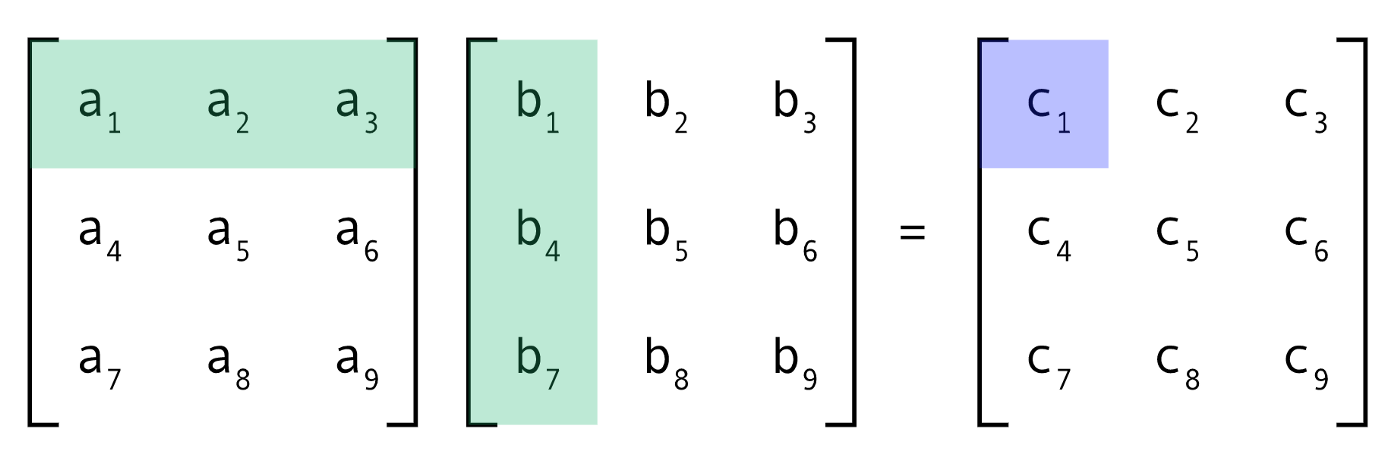
\includegraphics[width=0.5\linewidth]{producto_matrices}
	\caption{Esquema de la multipliación entre dos matrices, el producto escalar de los vectores resaltados en verde dan lugar al escalar marcado en azul. Se coge una fila de la primera matriz y una columna de la segunda. Debido a esto el producto de matrices no es conmutativo $AB\neq BA$.}
	\label{fig:productomatrices}
\end{figure}


Al multiplicar una matriz por un escalar (número), se multiplican todos los elementos de la matriz por ese escalar:
\begin{equation*}
	\begin{pmatrix}
		1 & 4  \\
		3 & 2
	\end{pmatrix}
	=
	\begin{pmatrix}
		5 \times (1) & 5\times (4)  \\
		5\times (3) & 5\times (2) 
	\end{pmatrix}
	=
	\begin{pmatrix}
		5 & 20  \\
		15 & 10
	\end{pmatrix}
\end{equation*}

\subsection{Determinantes}
El determinante es la variación el área/norma que causa una transformación lineal aplicada a una superficie/vector.

El determinantes de una matriz $(2\cross2)$ se calcula con la siguiente regla:
\begin{equation*}
	\det \begin{pmatrix} a & b \\
		c & d \end{pmatrix} = 
	\begin{vmatrix} a & b \\
		c & d \end{vmatrix} = ad - bc
\end{equation*}

Mientras que para una matriz $(3\cross3)$ se puede utilizar la expansión de Laplace\footnote{Muy útil para el cálculo de productos vectoriales entre vectores.}:
\begin{equation*}
	\begin{vmatrix}a&b&c\\ d&e&f\\ g&h&i\end{vmatrix} =
	a\begin{vmatrix}e&f\\ h&i\end{vmatrix} - b\begin{vmatrix}d&f\\ g&i\end{vmatrix} + c\begin{vmatrix}d&e\\ g&h\end{vmatrix}
\end{equation*}
Donde se puede utilizar cualquier columna o fila para expandir la matriz. Dependiendo de la cual, cambia el signo que tiene el determinante. Para un menor $M_{ij}$ el signo que tiene su elemento en la expansión es $(-1)^{i+j}$. Usualmente se da una matriz con un parámetro y se ha de tomar el determinante de esta, resultando en una ecuación de segundo grado normalmente. Es indispensable saber la expansión de Laplace. 

\subsection{Rango de una matriz}

El rango de una matriz es el máximo número de vectores independientes que se pueden sacar de la matriz, ja sean columnas o filas (y no una combinación de las dos). Se puede calcular el rango a partir del orden máximo de los menores no nulos de la matriz (cuando su determinante no es $0$).

Si hay en una matriz hay un menor no nulo de orden $k$ y todos los menores de orden $k+1$ son nulos, entonces el rango de la matriz es $k$. 

Conviene calcular el rango a través de la linealidad de las columnas o filas si se ve inmediatamente. No se pedirá calcular el rango de una matriz de mayor orden que 3.  

\subsection{Matriz inversa}
 $A^{-1}$ es la matriz inversa de $A$ si:
\begin{equation*}
	AA^{-1} = A^{-1}A = I
\end{equation*}
En otras palabras:
\begin{equation*}
	\exists A^{-1} \iff AA^{-1} = A^{-1}A = I
\end{equation*}
Se denomina matriz regular a una matriz que tiene inversa. 

\subsubsection{Cálculo de una matriz inversa}

Se puede calcular mediante la matriz adjunta:
\begin{equation*}
	A^{-1} = \frac{1}{|A|} (A^{\dagger})^{T}
\end{equation*}
Donde $A^{\dagger}$ es la matriz adjunta, definida mediante sus elementos como:
\begin{equation}
	m_{ij} = (-1)^{i+j}M_{ij}
\label{eq:matriz-adjunta}
\end{equation}

Para una matriz $A$ de orden $2$, su adjunta será:
\begin{equation}
	A^{\dagger} = \begin{pmatrix}
		a & b \\ c & d
	\end{pmatrix}^{\dagger} = \begin{pmatrix}
	d & -b \\ -c & a
\end{pmatrix}
\label{eq:2adjunt}
\end{equation}

Y para una matriz $A$ de orden $3$, su adjunta será:
\begin{equation}
	A^{\dagger} = \begin{pmatrix}
		a_{11} & a_{12} & a_{13} \\
		a_{21} & a_{22} & a_{23} \\
		a_{31} & a_{32} & a_{33}
	\end{pmatrix}^{\dagger} = \begin{pmatrix}
	+\begin{vmatrix} a_{22} & a_{23} \\ a_{32} & a_{33} \end{vmatrix} &
	-\begin{vmatrix} a_{21} & a_{23} \\ a_{31} & a_{33} \end{vmatrix} &
	+\begin{vmatrix} a_{21} & a_{22} \\ a_{31} & a_{32} \end{vmatrix} \\
	\\
	-\begin{vmatrix} a_{12} & a_{13} \\ a_{32} & a_{33} \end{vmatrix} &
	+\begin{vmatrix} a_{11} & a_{13} \\ a_{31} & a_{33} \end{vmatrix} &
	-\begin{vmatrix} a_{11} & a_{12} \\ a_{31} & a_{32} \end{vmatrix} \\
	\\
	+\begin{vmatrix} a_{12} & a_{13} \\ a_{22} & a_{23} \end{vmatrix} &
	-\begin{vmatrix} a_{11} & a_{13} \\ a_{21} & a_{23} \end{vmatrix} &
	+\begin{vmatrix} a_{11} & a_{12} \\ a_{21} & a_{22} \end{vmatrix}
\end{pmatrix}
\label{eq:3adjunt}
\end{equation}
Se pueden ver como el elemento de la fila $i$ y la columna $j$ es el menor $M_{ij}$ de la matriz $A$. El término $(-1)^{i+j}$ de la ecuación \ref{eq:matriz-adjunta} indica el signo que se le da a los menor dependiendo de la posición. No hace falta saber la ecuación \ref{eq:matriz-adjunta}, se puede aprender a hacer mecánicamente con la ecuación \ref{eq:3adjunt} y \ref{eq:2adjunt}. 

Haciendo la transpuesta de la adjunta y dividendo los componentes entre el determinante de la matriz original es como se calcula la inversa de esta. 

\subsection{Discusión de sistemas}

Los sistemas de ecuaciones se pueden representar mediante matrices: 
\begin{equation*}
	\begin{cases}
		px + y + z = 2\\
		2x + py + p^{2}z = 1\\
		2x + y + z = 2
	\end{cases} \rightarrow \left(\begin{array}{lll|l}
	p & 1 & 1 & 2 \\
	2 & p & p^{2} & 1 \\
	2 & 1 & 1 & 2
\end{array}\right)
\end{equation*}
Donde la última columna representa a que equivale la combinación lineal de los parámetros. Sin embargo siempre que se piensa a discurtir el sistema se prescinde de esta columna:
\begin{equation*}
	\left(\begin{array}{lll}
		p & 1 & 1 \\
		2 & p & p^{2} \\
		2 & 1 & 1 
	\end{array}\right)
\end{equation*}

Dependiendo del rango de estas matrices (denominando la primera como matriz ampliada), podemos diferenciar $3$ tipos de sistemas de ecuaciones:
\begin{enumerate}
	\item \textbf{Sistema Compatible Determinado}:\\
	
\end{enumerate}

\section{Geometría}
\section{Análisis}

\end{document}